%&pdflatex
\documentclass[final,leqno]{siamltex}
%\documentclass[10pt,onecolumn]{article}
\usepackage[top=2cm,bottom=3cm,left=3.5cm,right=3.5cm]{geometry}
\usepackage[utf8]{inputenc}
\usepackage{amsmath,amssymb,amsfonts,mathrsfs}
\let\proof\relax 
\let\endproof\relax
\usepackage{listings}
\usepackage{array}
\usepackage{mathtools}
\usepackage{dsfont}
\usepackage{graphicx}
\usepackage{pdfpages}
\usepackage[textsize=footnotesize,color=green]{todonotes}
\usepackage{algorithm, algorithmic}
\usepackage{array}
\usepackage{bm}
\usepackage{tikz}
\usepackage{subfigure}
\usepackage[normalem]{ulem}

%\usepackage{lineno}
%\pagewiselinenumbers
%\usepackage{uselinenofix}


\newcommand{\bs}[1]{\boldsymbol{#1}}

\newcommand{\equaldef}{\stackrel{\mathrm{def}}{=}}

\newcommand{\tablab}[1]{\label{tab:#1}}
\newcommand{\tabref}[1]{Table~\ref{tab:#1}}

\newcommand{\theolab}[1]{\label{theo:#1}}
\newcommand{\theoref}[1]{\ref{theo:#1}}
\newcommand{\eqnlab}[1]{\label{eq:#1}}
\newcommand{\eqnref}[1]{\eqref{eq:#1}}
\newcommand{\seclab}[1]{\label{sec:#1}}
\newcommand{\secref}[1]{\ref{sec:#1}}
\newcommand{\lemlab}[1]{\label{lem:#1}}
\newcommand{\lemref}[1]{\ref{lem:#1}}

\newcommand{\mb}[1]{\mathbf{#1}}
\newcommand{\mbb}[1]{\mathbb{#1}}
\newcommand{\mc}[1]{\mathcal{#1}}
\newcommand{\nor}[1]{\left\| #1 \right\|}
\newcommand{\snor}[1]{\left| #1 \right|}
\newcommand{\LRp}[1]{\left( #1 \right)}
\newcommand{\LRs}[1]{\left[ #1 \right]}
\newcommand{\LRa}[1]{\left\langle #1 \right\rangle}
\newcommand{\LRc}[1]{\left\{ #1 \right\}}
\newcommand{\LRb}[1]{\left| #1 \right|}

\newcommand{\tanbui}[2]{\textcolor{blue}{\sout{#1}} \textcolor{red}{#2}}
\newcommand{\Grad} {\ensuremath{\nabla}}
\newcommand{\Div} {\ensuremath{\nabla\cdot}}
\newcommand{\Nel} {\ensuremath{{N^\text{el}}}}
\newcommand{\jump}[1] {\ensuremath{\LRs{\!\left[#1\right]\!}}}
\newcommand{\uh}{\widehat{u}}
\newcommand{\fnh}{\widehat{f}_n}
\renewcommand{\L}{L^2\LRp{\Omega}}
\newcommand{\pO}{\partial\Omega}
\newcommand{\Gh}{\Gamma_h}
\newcommand{\Gm}{\Gamma_{-}}
\newcommand{\Gp}{\Gamma_{+}}
\newcommand{\Go}{\Gamma_0}
\newcommand{\Oh}{\Omega_h}

\newcommand{\eval}[2][\right]{\relax
  \ifx#1\right\relax \left.\fi#2#1\rvert}

\def\etal{{\it et al.~}}

\newcommand{\vect}[1]{\ensuremath\boldsymbol{#1}}
\newcommand{\tensor}[1]{\underline{\vect{#1}}}
\newcommand{\del}{\Delta}
\let\grad\relax
\newcommand{\grad}{\nabla}
\newcommand{\curl}{\grad \times}
\renewcommand{\div}{\grad \cdot}
\newcommand{\ip}[1]{\left\langle #1 \right\rangle}
\newcommand{\eip}[1]{a\left( #1 \right)}
\newcommand{\pd}[2]{\frac{\partial#1}{\partial#2}}
\newcommand{\pdd}[2]{\frac{\partial^2#1}{\partial#2^2}}

\newcommand{\circone}{\ding{192}}
\newcommand{\circtwo}{\ding{193}}
\newcommand{\circthree}{\ding{194}}
\newcommand{\circfour}{\ding{195}}
\newcommand{\circfive}{\ding{196}}

\def\arr#1#2#3#4{\left[
\begin{array}{cc}
#1 & #2\\
#3 & #4\\
\end{array}
\right]}
\def\vecttwo#1#2{\left[
\begin{array}{c}
#1\\
#2\\
\end{array}
\right]}
\def\vectthree#1#2#3{\left[
\begin{array}{c}
#1\\
#2\\
#3\\
\end{array}
\right]}
\def\vectfour#1#2#3#4{\left[
\begin{array}{c}
#1\\
#2\\
#3\\
#4\\
\end{array}
\right]}

%\newtheorem{proposition}{Proposition}
%\newtheorem{corollary}{Corollary}
%\newtheorem{theorem}{Theorem}
%\newtheorem{lemma}{Lemma}

\newcommand{\G} {\Gamma}
\newcommand{\Gin} {\Gamma_{in}}
\newcommand{\Gout} {\Gamma_{out}}
\newcommand{\insub}{{\rm in}}
\newcommand{\outsub}{{\rm out}}

\newtheorem{remark}{Remark}

\title{Notes on preconditioning for implicit CD systems}
\begin{document}

\maketitle

\section{Introduction}

A common approach to the numerical solution of the Navier-Stokes equations
\begin{align*}
\pd{u}{t} + u\cdot\grad u + \grad p &= f \\
\div u &= 0
\end{align*}
is to employ a splitting or projection method, where we 
\begin{enumerate}
\item compute an intermediate velocity $u^*$ by solving $$\frac{(u^*-u^k)}{dt} - \nu\Delta u^* = f(t^k)$$
\item correct the velocity by solving 
$$\begin{cases}
\frac{(u^{k+1}-u^*)}{dt} + \nabla p^k &= 0\\
\nabla \cdot u^{k+1} &= 0\\
u^{k+1}\cdot n &= 0 \quad \text{on the boundary}
\end{cases}$$
\end{enumerate}
This above step is the reason splitting schemes are referred to as projection methods - the weak form of (2) can be interpreted as the scaled $L^2$ projection of $u^*$ onto a divergence-free $u^{k+1}$ (after multiplying by a test function, $p$ can then be viewed as a Lagrange multiplier to enforce the divergence free constraint).  Since pressure is undetermined in the second step, we need to produce an approximation for $p$.  Based on the assumption that $\nabla \cdot u^{k+1}$ must be $0$, we can take the divergence of the second equation to get $$\nabla \cdot \frac{u^*}{dt} + \nabla\cdot \nabla p^k = 0,$$ which yields a Poisson equation for $p$ given $u^*$. 

The overall scheme is then 
\begin{enumerate}
\item Solve for $u^*$ through $$\frac{(u^*-u^k)}{dt} - \nu\Delta u^* = f(t^k)$$
\item  Solve for $p$ through $$\Delta p = \frac{1}{dt}\nabla \cdot u^*$$
\item Solve for $u^{k+1}$ through $$\frac{(u^{k+1}-u^*)}{dt} + \nabla p^k = 0.$$
\end{enumerate}
Note that both steps 2 and 3 involve the solution of a Poisson and $L^2$-projection problem, respectively, both of which involve symmetric, positive-definite operators which can be solved very efficiently in a scalable fashion.  However, as step 1 involves the solution of a non-symmetric convection-diffusion system, the full system is often eschewed in favor of a second splitting, where the convective term is updated explicitly, and diffusion accounted for implicitly.  

A particularly restrictive aspect of this solution method is the CFL condition for spectral finite elements
\[
dt < O\LRp{\LRb{u}\frac{h}{N^2}},
\]
which results from the $O(1/N^2)$ minimum spacing between the GLL nodes of order $N$ on a given element.  For high $N$ ($N>20$ and higher), the explicit CFL condition can be incredibly restrictive.  Our aim is to consider instead the direct solution of the convection-diffusion system, which we hope will allow us to loosen the CFL restriction.  

\section{Scalar convection-diffusion}

We investigate first the scalar convection-diffusion-reaction equation with homogeneous Dirichlet boundary condtions.  
\begin{align*}
u + \div(\beta u) - \epsilon \Delta u &= f\\
\left.u\right|_{\Gamma} = 0,
\end{align*}
and preconditioning strategies for systems resulting from high order spectral element discretizations of this equation.  

\subsection{1D experiments}

Effective preconditioning of convection-diffusion systems has often exploited the physics of convection-dominated problems.  The relevant physics are often encapsulated in the Greens function, which has been effectively used in the preconditioning of systems resulting from discretizations of convection-diffusion problems.  The idea put forth in \cite{Loghin97,Loghin99} is that the support of the Green's function in the convection-dominated limit is purely upstream.  Under a ``with-the-flow'' ordering of the degrees of freedom, the matrix inverse becomes lower triangular.  Loghin and Wathen take advantage of this by using a Gauss-Seidel preconditioner on both uniform and adaptive meshes of linear and bilinear elements.  

\begin{figure}
\subfigure[Greens function for $\epsilon = 1.0$]{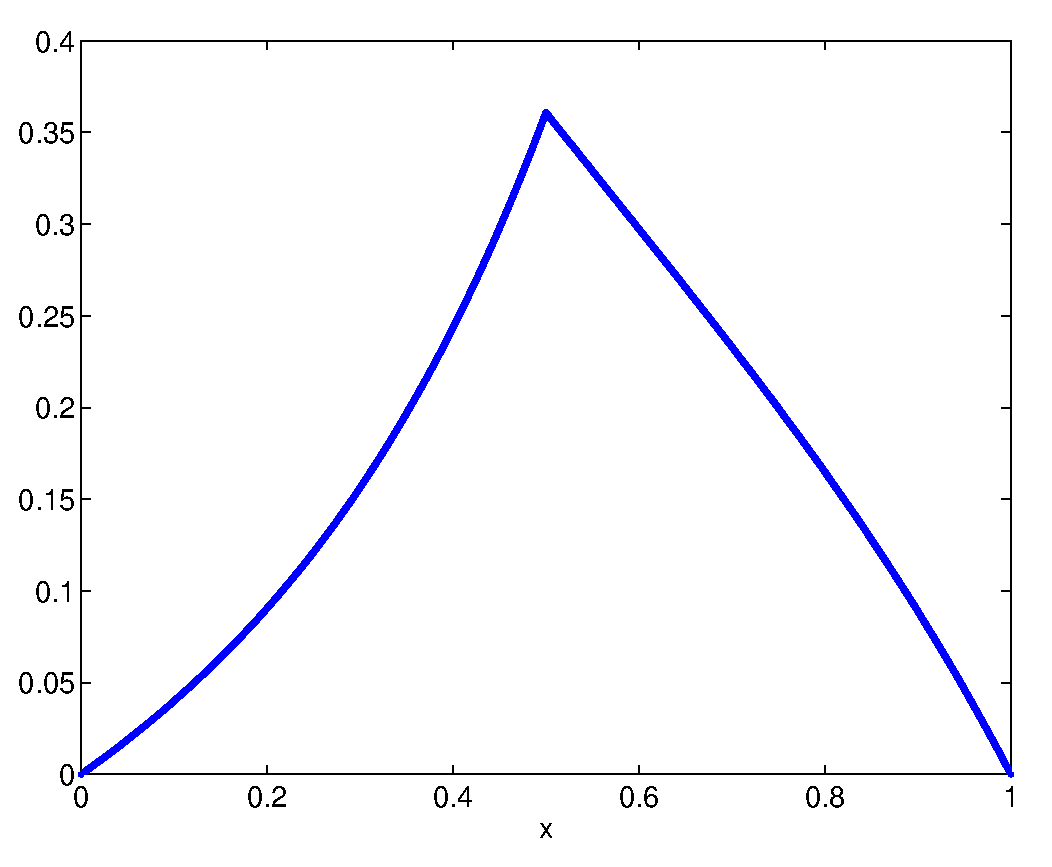
\includegraphics[width=.47\textwidth]{g_eps1.eps}}
\subfigure[Greens function for $\epsilon = 10^{-2}$]{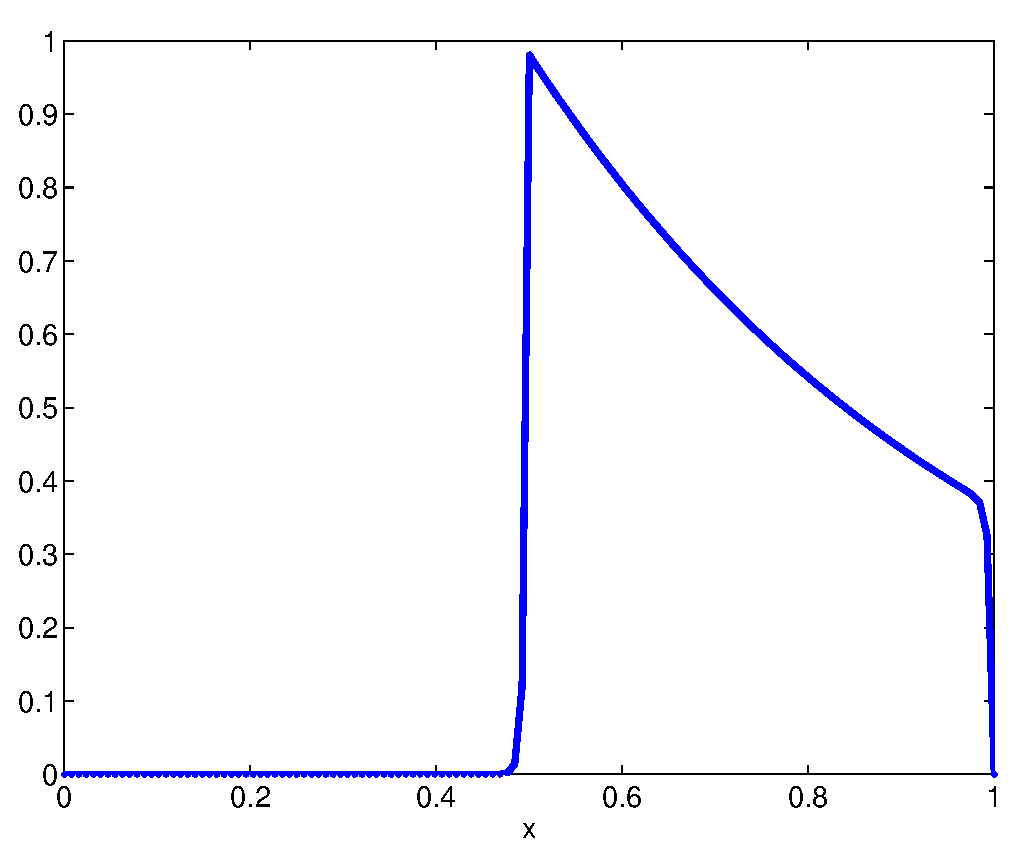
\includegraphics[width=.47\textwidth]{g_eps100.eps}}
\caption{Greens functions for diffusive/convective regimes.}
\end{figure}

A requirement for use of the Gauss-Seidel preconditioners for the convection-diffusion problem is a discretization that is stable in the convective limit; to this end, they employ SUPG stabilization in all their examples.  

\subsubsection{Resolved meshes and higher order elements}

Unfortunately, the Gauss-Seidel preconditioner relies on the fact that the support of the convection-diffusion Green's function in the cross and downstream directions decays to zero over a distance of roughly $\epsilon$; this implies that, for resolved meshes where $h\approx \epsilon$, a ``with-the-flow'' preconditioner does not work as effectively as with under-resolved meshes.  Figure~\ref{fig:resolved_GS} shows GMRES convergence in these two cases; for $h/\epsilon < 1$, convergence is relatively fast; for $h/\epsilon = O(1)$ or larger, the convergence rate suffers.  

\begin{figure}
\subfigure[Under-resolved convergence for $\epsilon = 10^{-6}$]{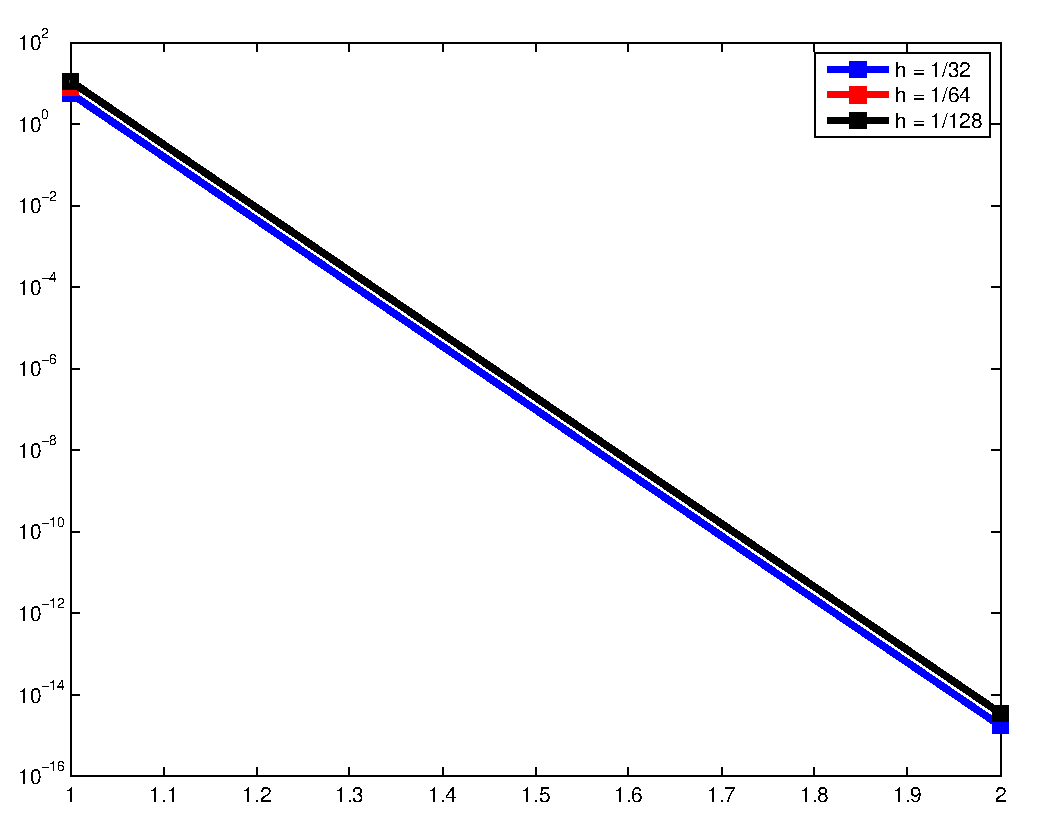
\includegraphics[width=.47\textwidth]{GS_underResolved.eps}}
\subfigure[Resolved convergence for $\epsilon = 10^{-2}$]{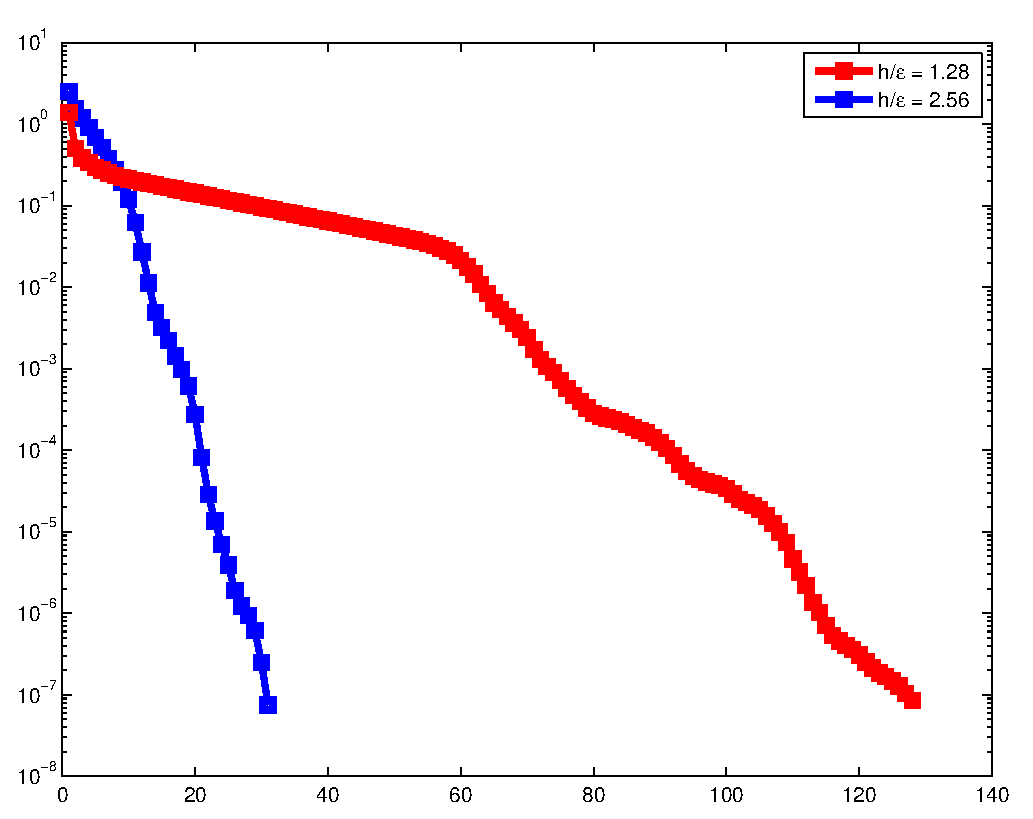
\includegraphics[width=.47\textwidth]{GS_resolved.eps}}
%\subfigure[GMRES convergence]{\includegraphics[width=.47\textwidth]{GS_higherOrder.eps}}
\caption{GMRES convergence for resolved and under-resolved linear meshes.}
\label{fig:resolved_GS}
\end{figure}

Higher order elements display similar issues 

\begin{figure}
\subfigure[Under-resolved convergence for $\epsilon = 10^{-6}$]{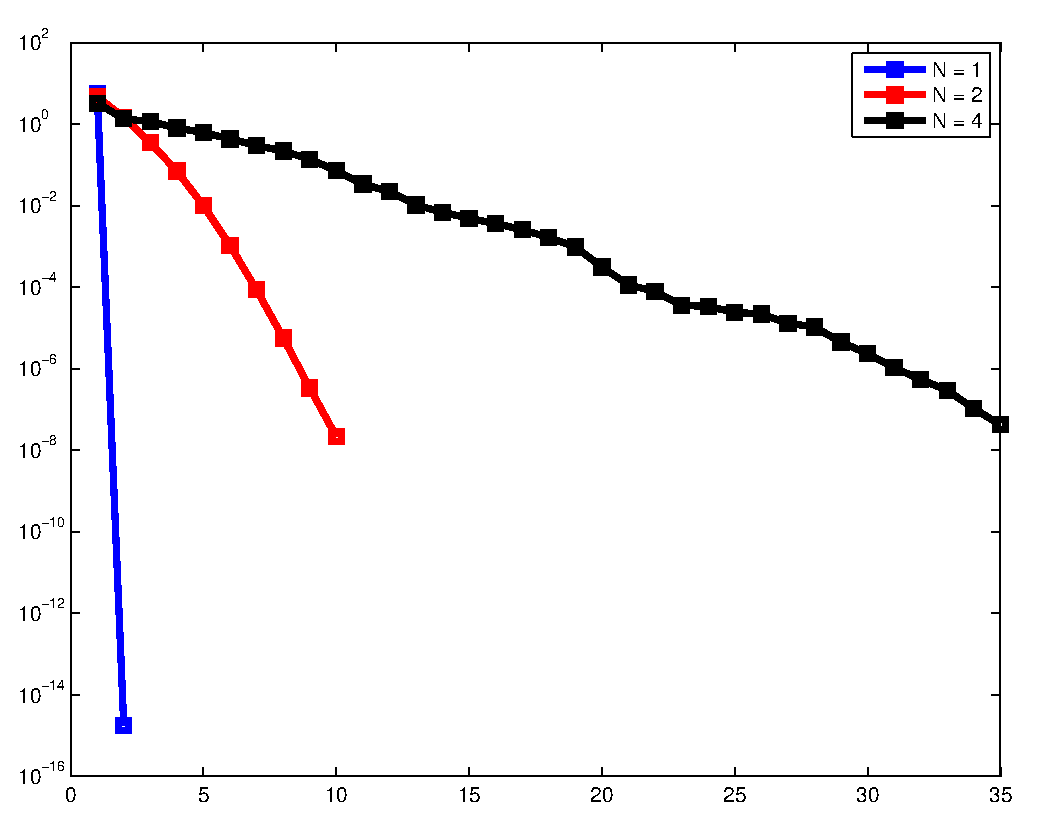
\includegraphics[width=.47\textwidth]{GS_HO_underResolved.eps}}
\subfigure[Resolved convergence for $\epsilon = 10^{-2}$]{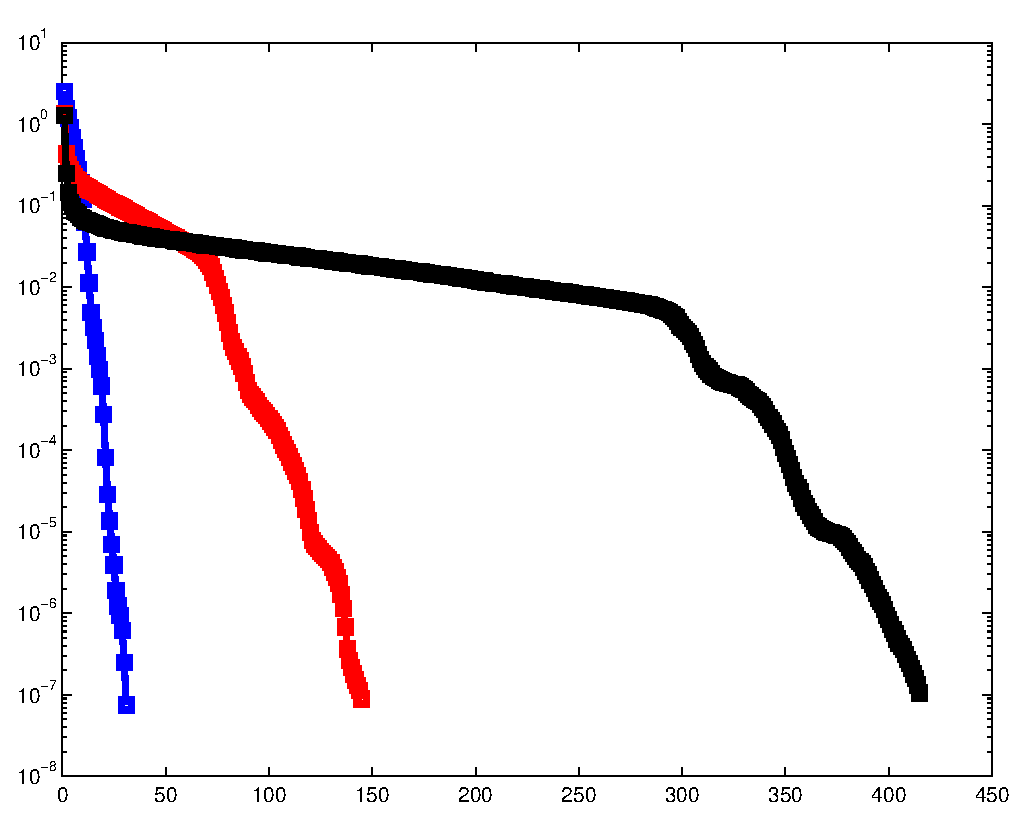
\includegraphics[width=.47\textwidth]{GS_HO_resolved.eps}}
%\subfigure[GMRES convergence]{\includegraphics[width=.47\textwidth]{GS_higherOrder.eps}}
\caption{Greens functions for diffusive/convective regimes.}
\label{fig:rHO_GS}
\end{figure}

\subsubsection{Schur complement downwinding}

\cite{Cai14}
\begin{enumerate}
\item Show Wathen preconditioning breaks down for no stabilization
\item Show Wathen preconditioning breaks down for resolved meshes
\item Show Wathen preconditioning breaks down for higher order
\item Analyze static condensation case
\item Addition of a mass matrix (with mass vector).  
\end{enumerate}

\subsection{2D experiments}

Todos
\begin{enumerate}
\item Document current AGMG verification ($h$ and $N$ independence)
\item Compare AGMG/Wathen downwind GS
\item Analyze static condensation case
\item Implement $A+A^T$ AGMG coarsening
\end{enumerate}

\subsection{AGMG}

\subsubsection{Static condensation}

Static condensation involves the representation of interior degrees of freedom (nodes in the interior of an element) in terms of globally coupled degrees of freedom through the local Schur complement.  

Todos
\begin{enumerate}
\item Try iterative solver on single element system - how do you do matrix-free condensation?  
\item Balance cost - what is the baseline?  Can we do a GPU workgroup implementation?  
\end{enumerate}


\bibliographystyle{unsrt}
\bibliography{main}

\end{document}